 \chapter{Теоретическая часть}

\section{Модель микросервиса}

К каждому микросервису выделяются общие функциональные требования:
\begin{itemize}
  \item При необходимости выполнять CRUD операции с базой данных
  \item При необходимости писать сообщения в логброкер сообщений
  \item При необходимости читать сообщения из логброкера сообщений
\end{itemize}

К каждому микросервису выделяются общие нефункциональные требования:
\begin{itemize}
  \item Соответствовать чистой архитектуре
  \item Иметь высокий cohesion и низкие coupling
\end{itemize}


Исходя из этих требований, типовая архитектура нашего сервиса будет соответствовать приведенной.

\begin{figure}[H]%
	\begin{center}
		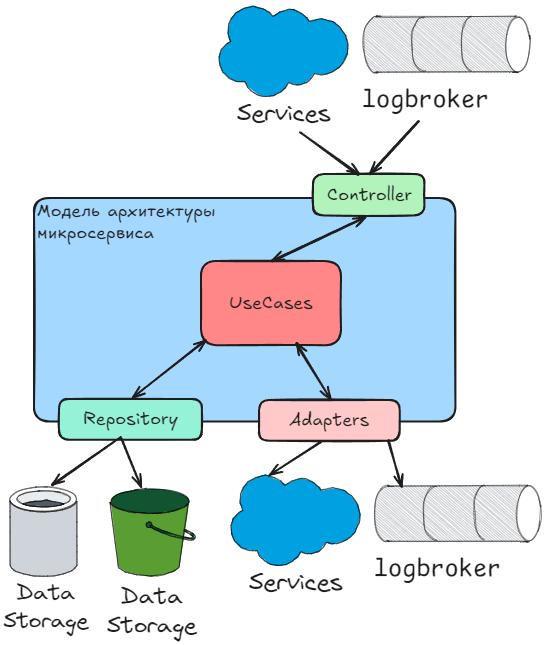
\includegraphics[width=.5\columnwidth]{./img/tipovoy_micric.png}%
	\end{center}
	\caption{Модель типового микросервиса}%
	\label{pic:tipovoy_micric}%
\end{figure}

\section{Модели модулей системы}
\subsection{Модель сервиса аутентификации}

Микросервис аутентификации осуществляет регистрацию новых пользователей, и обновление токенов у уже существующих.
Для сущесвующих пользователей он выдает новую пару JWT tokens(access token + refresh token) по refresh token или логину
и паролю.

Функциональные требования к сервису аутентификации:
\begin{itemize}
  \item Возможность регистрировать новых пользователей в сервисе
  \item Подписывать JWT ключи для авторизации
  \item Обменивать логин пароль или refresh JWT ключ на новый resfresh JWT ключ
\end{itemize}

Тогда для соответствия требованиям, модель базы данных:
\begin{figure}[H]%
	\begin{center}
		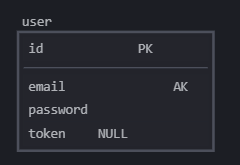
\includegraphics[width=.5\columnwidth]{./img/auth_db_model.png}%
	\end{center}
	\caption{Модель базы данных сервиса аутентификации}%
	\label{pic:auth_db}%
\end{figure}


Для обмена refresh token на новую пару ключей, в токен необходимо зашивать ID пользователя.
В соответствии с требованиями, модель сервиса авторизации:
\begin{figure}[H]%
	\begin{center}
		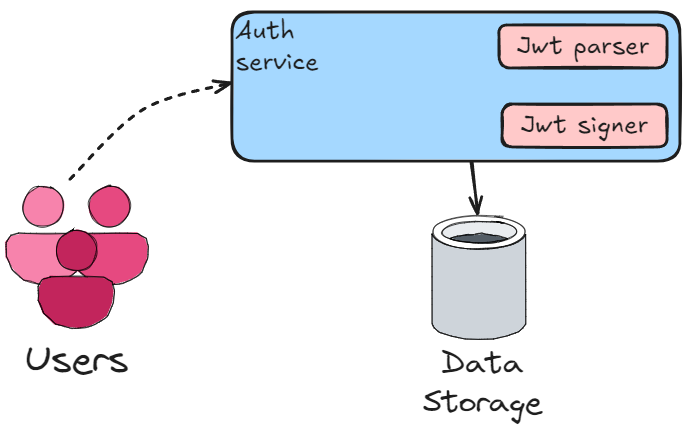
\includegraphics[width=.5\columnwidth]{./img/auth_model.png}%
	\end{center}
	\caption{Модель сервиса аутентификации}%
	\label{pic:auth_model}%
\end{figure}


\subsection{Модель сервиса узи}
Для начала нужно определить вид данных которые должен хранить узи.

Узи представляет из себя последовательный набор кадров, конкретной щитовидной железы. На щитовидной
железе могут быть обнаружены злокачественные образования, называемыми \textbf{узлами}. Узел злокачественного образования
может быть запечатлен на нескольких кадрах, такое отображения узла на конкретном кадре называется \textbf{сегмент}ом,
узлов может быть любое количество. Каждый узел и сегмент в отдельности характеризуется классификационными признаками.
На данный момент имеется 3 классификациооных признака: вероятности принадлежности узлов к классам \textbf{TI-RADS}.
TI-RADS, описывает стадию злокачественного образования, существует 3 стадии: TI-RADS23, TI-RADS4, TI-RADS5.

Функциональные требования к сервису узи:
\begin{itemize}
  \item Принимать единуб композицию кадров узи, разбивать и сохранять ее по кадрам.
  \item После разбиения узи по кадрам, оповещать через брокер сообщений, сервис с ml моделью, о доступности обработки изображения
  \item Предоставлять возможность совершать CRUD операции над узлами, сегментами, узи, ti-rads, images.
  \item Сохранять результат сегментации и классификации нейронной моделью посредством логброкера сообщений.
\end{itemize}


Тогда для соответствия требованиям, модель базы данных:
\begin{figure}[H]%
	\begin{center}
		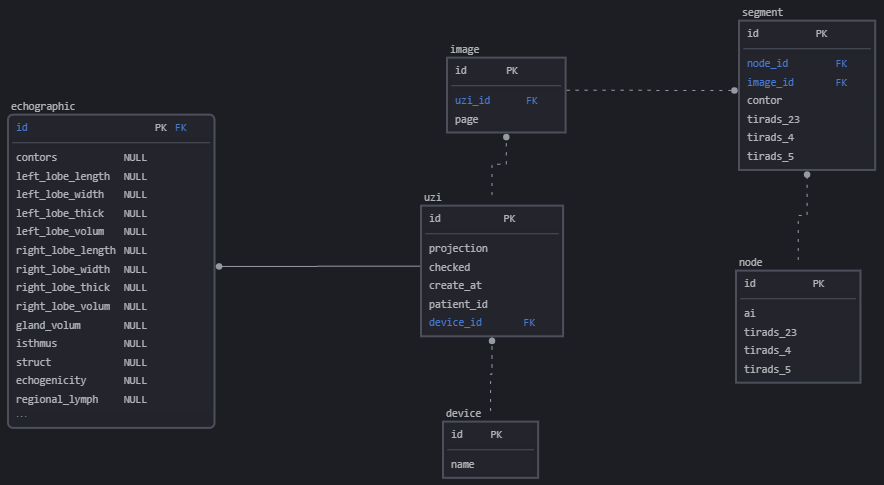
\includegraphics[width=.5\columnwidth]{./img/uzi_db_model.png}%
	\end{center}
	\caption{Модель базы данных сервиса аутентификации}%
	\label{pic:auth_db}%
\end{figure}


В соответствии с требованиями, модель сервиса узи:
\begin{figure}[H]%
	\begin{center}
		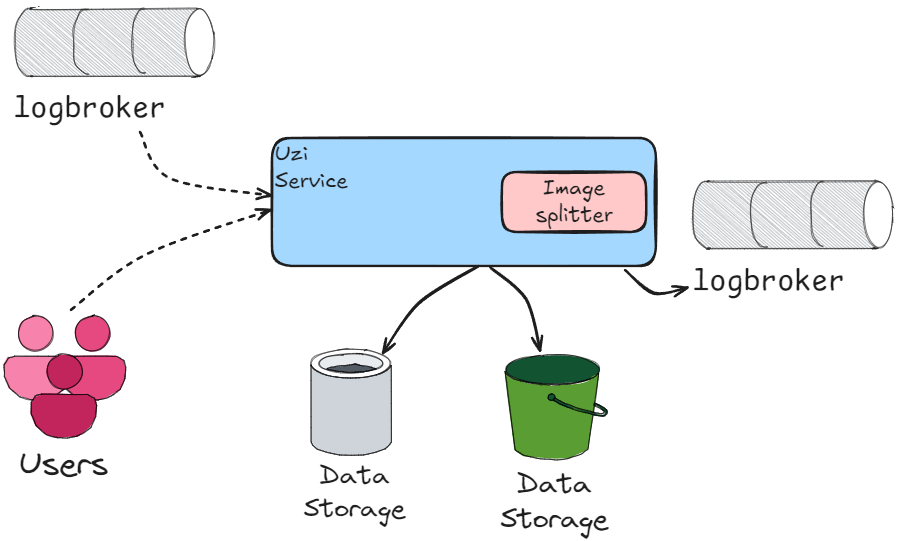
\includegraphics[width=.5\columnwidth]{./img/uzi_model.png}%
	\end{center}
	\caption{Модель сервиса УЗИ}%
	\label{pic:auth_model}%
\end{figure}


\subsection{Модель Gateway API}
Сервис gateway API, является точной входа для всех пользователей системы. Сервис делает запросы в дочерние микросервисы.


Функциональные требования к сервису Gateway API:
\begin{itemize}
  \item Если дочерний микросервис реализует публичный для пользователя контракт взаимодействия, то сервис должен реализовывать доступ к этому контракту для пользователя
  \item Предоставлять пользователю по запросу кадры узи
  \item Запускать пайплайн обработки узи, посредством сообщения в логброкер
\end{itemize}


В соответствии с требованиями, модель сервиса Gateway:
\begin{figure}[H]%
	\begin{center}
		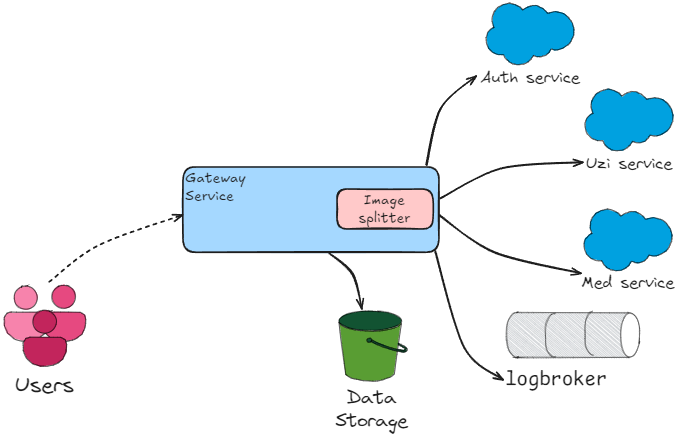
\includegraphics[width=.5\columnwidth]{./img/gateway_model.png}%
	\end{center}
	\caption{Модель сервиса gateway}%
	\label{pic:auth_model}%
\end{figure}

% В этой главе описываются разработанные/модифицированные модели/методы/
% алгоритмы, или/и описывается применение известных стандартных методов. Также, 
% в конце главы обычно приводится общая архитектура программной системы, 
% вытекающая из описанной теории. Приведенные ниже заголовки подразделов так же 
% весьма примерные и сильно зависят от особенностей конкретной работы.

% Формулы и их части необходимо набирать в математическом режиме
% (символ \verb|$|). Во избежание переноса длинных формул между строками их 
% стоит размещать по центру колонки, например,
% \begin{center}
% $S a b c = (\lambda x y z. x z (y z)) a b c = a c (b c)$,
% \end{center}
% \noindent и, если абзац после формулы продолжается, необходимо использовать 
% \verb|\noindent|.

% Для набора правил вывода можно использовать пакет \texttt{mathpartir.sty}. 
% Правила вывода могут быть вынесены в виде рисунка (см. рис. 
% \ref{img:inferrules}).

% \begin{figure}[t]
%   \centering
%     \begin{mathpar}
%       \inferrule{
%         M \to M'
%       }{
%         N M \to N M'
%       } \quad (\mu) \and 
%       \inferrule{
%         M \to M'
%       }{
%         M N \to M' N
%       } \quad (\nu) \and
%       \inferrule{
%         M \to M'
%       }{
%         \lambda x. M \to \lambda x. M'
%       } \quad (\xi)
%     \end{mathpar}
%   \caption{Правила редукции}
%   \label{img:inferrules}
% \end{figure}

% Для оформления определений, теорем, доказательств и т.~п. могут быть 
% использованы соответствующие окружения, например:

% \begin{definition}
% (высказывание)
% Высказыванием называется любое истинное или ложное утверждение.
% \end{definition}


% \section{Модель системы \dots}

% \dots




% \section{Метод решения задачи для \dots}

% \dots





% \section{Алгоритмы вычисления \dots}

% \dots





% \section{Обобщенная архитектура и интерфейсы \dots}

% В ряде случаев, все или некоторые результаты проектирования могут быть представлены во второй главе. Обычно же архитектура описывается в третьей главе.

% \section{Выводы}

% Необходимо перечислить, какие теоретические результаты были получены с 
% указанием степени новизны. Например: <<Была разработана такая-то модель. Она 
% представляет собой адаптированную версию модели $X$, в которой уравнение $Z$ 
% заменено на уравнение $Z'$>>. Еще пример: <<Была предложена такая-то 
% архитектура, она отличается от типовой в том-то и том-то. Это позволяет 
% избежать таких-то проблем.>>. При этом не следует заниматься <<высасыванием из 
% пальца>>: <<Поставленная задача является типовой; для ее решения применены 
% стандартные средства (перечислить, какие).>>.

%%% Local Variables:
%%% TeX-engine: xetex
%%% eval: (setq-local TeX-master (concat "../" (seq-find (-cut string-match ".*-3-pz\.tex$" <>) (directory-files ".."))))
%%% End:
